%************************************************
\chapter{Related Work}\label{ch:related}
%************************************************
\markboth{Related Work}{Related Work}

This document describes perceptually optimized video processing systems, ranging from energy-constrained mobile cameras to cloud video storage infrastructure. I first present a survey of related work in hardware and software support for video systems, from mobile devices to cloud video computing. I then organize relevant works based on their use of the perceptual optimizations we consider in this thesis: structural, semantic, or saliency-based.

\begin{figure*}[h]
\centering
    \begin{center}
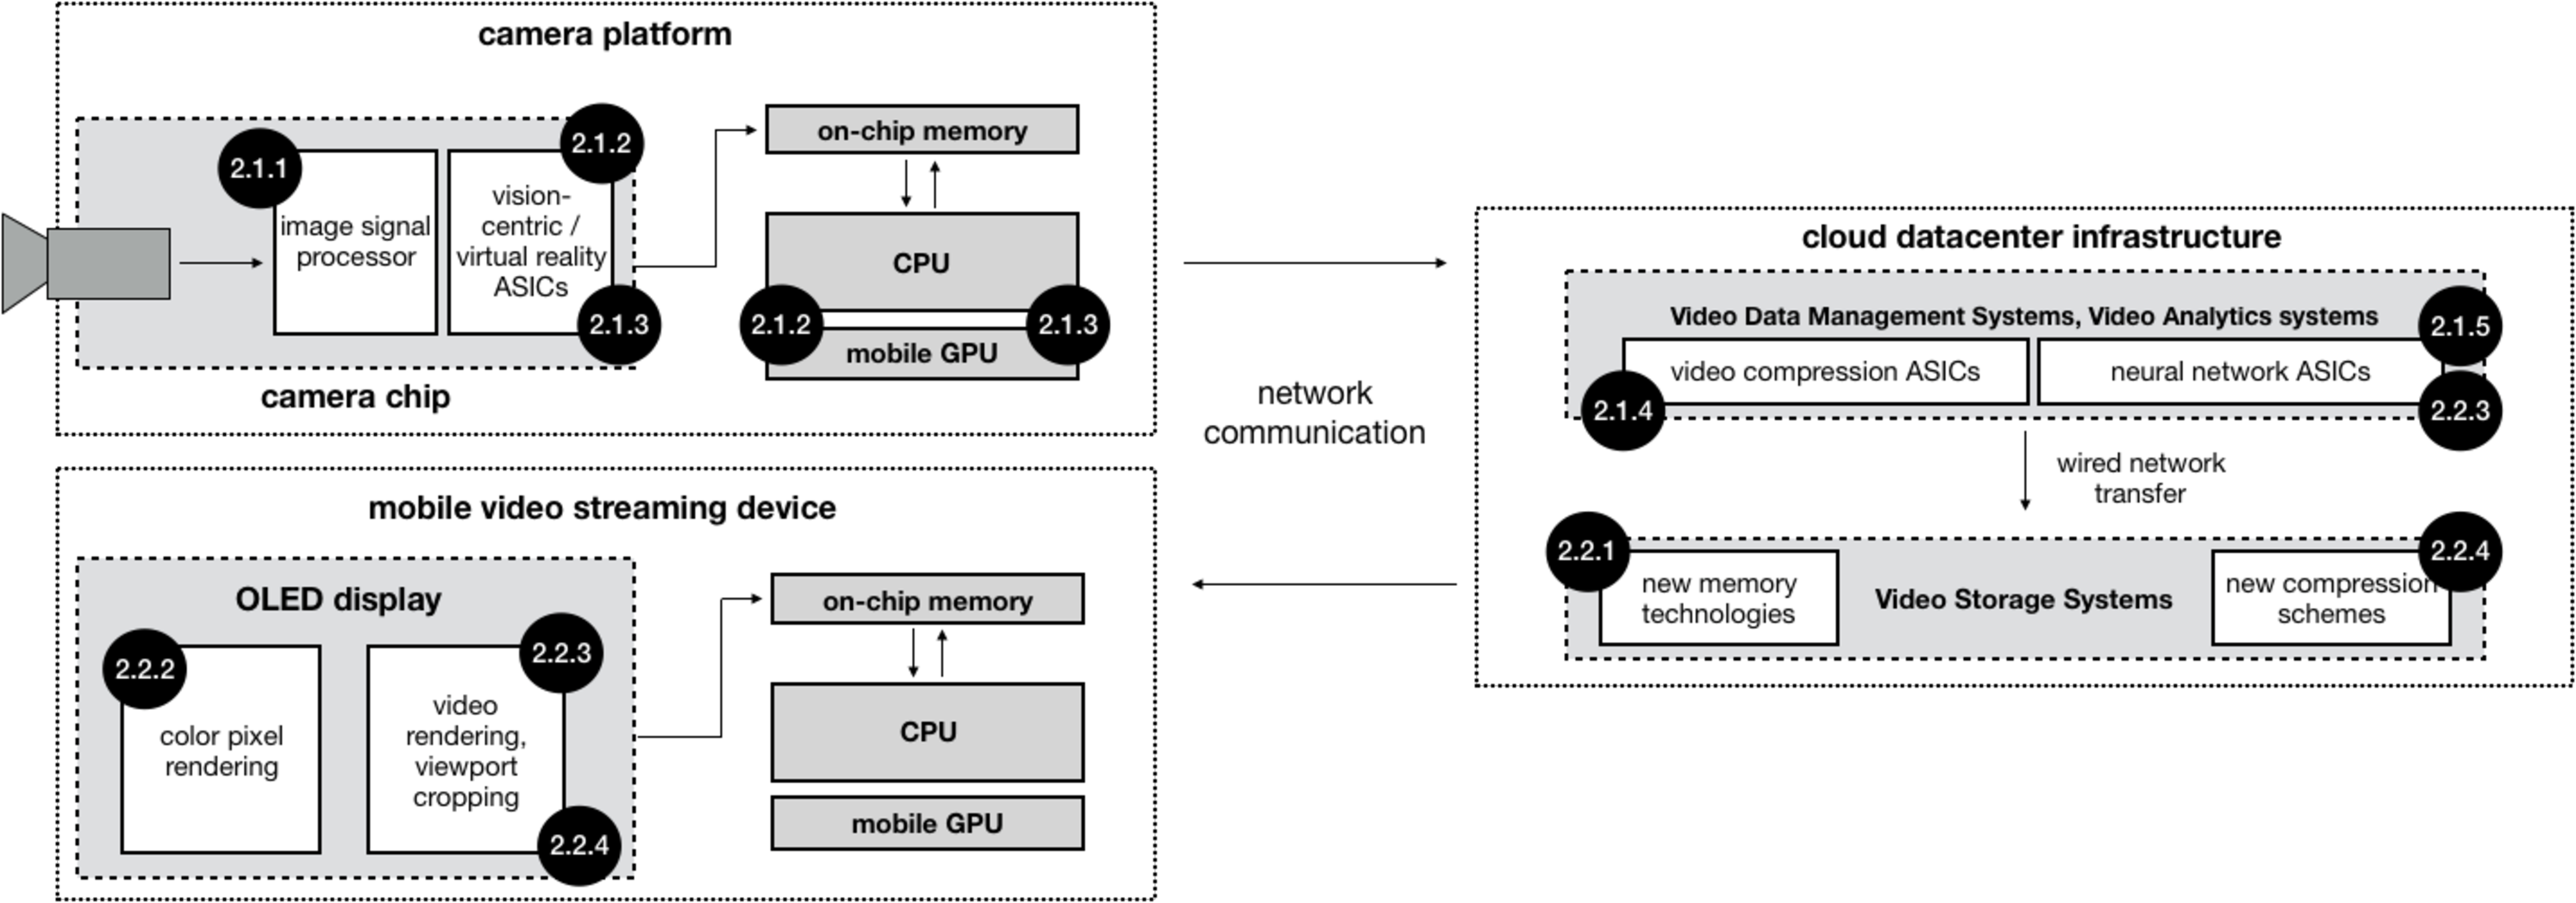
\includegraphics[width=\textwidth]{hfbs-figs/generals-related-work.pdf}
    \end{center}
    \caption{This document's related work covers research in visual computing systems spanning capture, processing, and storage. Prior work related to camera capture hardware, including near-sensor accelerators, vision-centric accelerators, and on-camera acceleration, is discussed in~\ref{sec:related:camera},\ref{sec:related:vision-hw}, and \ref{sec:related:vr-hw}. Related work on cloud datacenter infrastructure for visual computing is discused in \ref{sec:related:streaming} and \ref{sec:related:vdbms}. A key concern for this thesis is minimizing data movement and overall data bandwidth both within the delineated platforms and across them.}
    \label{fig:related-work}
\end{figure*}


\section{Systems and Architecture for Visual Computing}

\subsection{Near-sensor processing for camera capture}
\label{sec:related:camera}

Image sensor data is typically captured as an analog signal and then converted to a digital signal for processing.
Recent work investigated how to improve image capture efficiency by moving preliminary processing into the analog domain at the sensor node.
Centeye chips~\cite{Centeye}, for instance, allow arbitrary analog computations on the sensor signals.
Other work studied computing early layers of convolutional NNs at the pixel level~\cite{Chen_2016_ASPVision, redeye, conv-sens09}.
In addition to the analog domain, these early compute stages can be implemented in the mixed-signal domain, using techniques like stochastic computing~\cite{stoch-edge-sensor14, Alaghi13}.

\subsection{Vision-centric specialized hardware accelerators}
\label{sec:related:vision-hw}

After visual data is captured and converted into a digital signal at the sensor node, it is sent through an image sensor processor (ISP).
The rise of computer vision and computational photography has inspired a number of computer architectures to support image processing as well as more complex functionality.
Flexible vision architectures~\cite{convolution_engine, clemons_eva, clemons_pmem, hpca_visionsys, vasilyev_2016} provide higher performance for image processing and vision applications while maintaining programmability.
One commercial vision processor, Movidius's Myriad 2 processor~\cite{myriad15}, has 20 hardware accelerators supporting a number of image processing kernels as well as GPU-like accelerators and a RISC core.
The Frankencamera~\cite{adams2010frankencamera} is a software-programmable camera architecture integrated with the camera design and form factor.
Mobile SoCs such as TI's OMAP, Nvidia's Tegra, and Qualcomm's Snapdragon provide image processing functionality as well as programmable computation for mobile cameras~\cite{omap,tegra,snapdragon}.

Hardware acceleration for specific vision applications is also well-explored to provide faster performance or more energy efficiency: these include face detection on FPGAs~\cite{cvpr2007, cho_parallelized_2009} and GPUs~\cite{vj_gpu}, and neural network vision accelerators on ASIC, FPGA, and GPU platforms~\cite{farabet2010, neuflow,snnap,nn_fpga,nsp_iscas,bilat_isscc,myriad15,convolution_engine,shidiannao,minerva,eyeriss,buckler2018eva2}.
These implementations explore performance tradeoffs across parallelized configurations of processing elements, using different hardware substrates or data movement techniques to improve speed or energy efficiency.

Recent work addresses energy efficiency of mobile video compression as a critical workload as well.
Finchelstein~\etal evaluate the impact of parallel decoder cores on a \avc chip design~\cite{multicore-avc}.
Tikekar \etal contribute a related parallel video decoder design using embedded DRAM to reduce data movement for VR devices~\cite{tikekar18ijssc}.
Boroumand \etal evaluate executing video decode hardware with processing-in-memory (PIM) to reduce energy from data movement~\cite{google2018asplos}.

Instead of designing custom hardware to support specialized vision computation, another approach is to offload image processing computation from mobile devices to the cloud, where compute resources are more plentiful and programmability is more flexible~\cite{pervasive_compute}.
Forchheimer and Astrom~\cite{Forchheimer94} discuss in-sensor image processing as a method to reduce image sensor data to useful information by performing pre-processing.
Cuervo et al. use computation offloading to accelerate complex processing on mobile devices~\cite{cuervo2010maui}.
Gharbi et al. use computation offloading techniques to rapidly apply image filters while saving energy~\cite{transform_recipes}.
But in recent years, the opposing case for ``onloading'' computation (i.e., migrating the computation back to the sensor) has grown more popular, due to the exponential growth in raw image sensor data and network communication costs as well as privacy concerns~\cite{han-hotos, likamwa-apsys}.
Barr and Asanovi\'{c} observed that naive lossy compression can needlessly increase energy consumption for offloading if it is more expensive than computing on-device~\cite{barr_asanovic}.
Han et al. use sensor-based filters to reduce the size of data to be processed on-device to make onloaded computation feasible~\cite{glimpsedata}.
Our hardware-software codesign approaches explore the tradeoff space between offloading and onloading in the context of highly constrained camera systems.

\subsection{Hardware accelerators for virtual reality video capture}
\label{sec:related:vr-hw}

There are many ways to capture and render VR video, but each method presents unique challenges.
Light fields ~\cite{levoy1996light}, a type of image that conveys information about the flow of light in a scene, are the most general and immersive solution to VR imagery.
Proposed light field-based capture systems, however, require an enormous amount of input and output data, and rendering on the client side is compute-intensive.
While impressive results for light field images have been demonstrated in VR ~\cite{Huang2015}, video is a greater challenge.

Other solutions for immersive video viewing, such as free-viewpoint video ~\cite{carranza2003free} and concentric mosaics ~\cite{shum2005virtual}, are also challenging to process and display using standard video formats, resulting in systems that are not yet stable enough to motivate hardware support.
In contrast, the Jump VR video system~\cite{googlejump} is designed to be practical to compute, edit, and stream.
Processing the 16 camera video array requires computing optical flow between images from each adjacent pair of cameras and then interpolating the images to produce the \emph{omnidirectional stereo} projection~\cite{peleg2001}.
The output is a pair of equirectangular spherical video streams, one stream for the left eye and one stream for the right.
Anderson et al. ~\cite{googlejump} employ a bilateral-space solver for optical flow to efficiently produce high quality edge-aware flow results that are well-suited to omnidirectional stereo image interpolation.
They observe that the majority of rendering time is spent running the bilateral solver.
Modern systems using similar pipelines require users to upload camera streams to a cloud service or high-performance computing system---this workflow impedes real-time applications such as live VR video streaming.
While real-time hardware systems for processing VR video are becoming commercially available~\cite{gopro,sphere,vahana}, these existing solutions provide either live panorama processing or stereoscopic 3D, not both.

Most similar to the design discussed in~\ref{ch:hfbs} is that of Rithe et al.~\cite{bilat_isscc}, who designed a low-power reconfigurable processor for bilateral filtering.
Their design differs by implementing the splatting and slicing operations in hardware, but it can only perform streaming bilateral filters and does not support repeated iterations of filtering in-memory, a necessity for fast bilateral-space optimization.

\subsection{Video streaming and storage systems}
\label{sec:related:streaming}

The rise of video sharing applications has driven significant recent work in processing and storage systems for video content.
An early example, the Stony Brook Video Server, codesigned its video streaming infrastructure with disk storage to deliver real-time video streaming for early Internet architectures~\cite{vernick1996stonybrook}.
Since then, video systems have specialized for subdomains like social media, entertainment, and video streaming.
Social media services like Facebook or YouTube distribute user-uploaded content from many types of video capture devices to many types of viewing devices, typically serving a small number of popular or livestreamed videos at high quality and low latency, as well as a long tail of less popular videos~\cite{fblive, tang2017popularvid}.
These workloads motivated the introduction of custom media storage infrastructure and fault-tolerant frameworks for processing video uploads at scale~\cite{beaver2010haystack, muralidhar2014f4, huang2017sve, vbench}.
Entertainment platforms like Netflix and Amazon Video have smaller amounts of video data than social media services, but incur significantly more network traffic to distribute videos broadly.
These services maintain user experience by transcoding videos at high quality for a range of heterogeneous devices and bitrate requirements, tailoring encode settings by title, streaming device, and video scene~\cite{netflix2016mobilecoding,netflix2015pertitle,netflix2018dynamicopt,netflix2018shotbased}.

Recent systems work has proposed new designs for datacenter-scale video transcoding and streaming infrastructure, specifically optimized for the large data bandwidth and many streaming endpoints typical of modern video workloads~\cite{fouladi2017excamera, fouladi2018salsify,liu2016greenvid, asicclouds}.
These systems codesign compute and network layers with software implementations of typical video transcoding steps to better leverage datacenter resources, working within the bounds of existing video compression or streaming application requirements.

\subsection{Cloud video management and analytics}
\label{sec:related:vdbms}

While systems for optimizing cloud-scale transcoding are well studied, more recent focus on pushing video content through complex analytics and processing pipelines has motivated a resurgence of interest in video database management systems (VDBMSs).
Early systems focused primarily on supporting image search queries and content-based image retrieval, with workloads on the order of a thousand images~\cite{ogle1995chabot, faloutsos1994efficient, carson1999blobworld, chaudhuri1996optimizing, visualrank}.
In comparison with the earlier VDBMS designs, these more recent VDBMSs have dramatically increased their supported workload sizes and domains supported, such as for a wide range of deep learning for video analytics and computational photography workloads, as well as compressed video and light field data formats. These VDBMSs include Scanner~\cite{poms2018scanner}, LightDB~\cite{lightdb}, NoScope~\cite{noscope}, BlazeIT~\cite{blazeit}, DeepLens~\cite{deeplens}, Chameleon~\cite{chameleon18sigcomm},  Focus~\cite{focus18osdi}, Optasia~\cite{optasia2016lu}, Tahoma~\cite{anderson2018physical} and VideoStorm~\cite{videostorm}.
Prior work has also evaluated using hardware acceleration~\cite{asicclouds, liu2016greenvid, vbench} in the cloud to improve video processing performance.


\section{Perceptual Optimizations for Visual Computing}

\subsection{Approximate visual computing}
Approximate computing research seeks to trade off computation and energy consumption for quality.
The key value proposition is that many application domains, such as visual computing, can tolerate small drops in quality for benefits in speed or energy efficiency~\cite{8054698, sampson2011enerj}.
While much of the literature considers image and video processing a natural domain for evaluating general-purpose approximate computing techniques, the metrics for evaluation are restricted to per-pixel quality metrics, as opposed to higher-level quality information~\cite{sampson2011enerj,snnap,Guo:2016:HIS:2872362.2872413,8342234}.
A notable exception to this is approximate computing work targeted at machine learning applications, which measures precision and recall for frames or different video segments~\cite{snnap}.
Approximate computing techniques have been specifically applied to video processing~\cite{xu2018videochef} and storage~\cite{jevdjic2017approxvid} in support of conventional video compression algorithms, as well.
While these techniques are in the spirit of trading off quality for visual computing performance, they either focus only on pixel-level optimizations or are more general-purpose and coarse than the perceptual optimizations considered for this thesis.

\subsection{Structural video data optimization}
Structural perceptual information refers to the physical structure of the visual data (e.g., spatial location, depth perception, color spaces).
While these attributes exist or can be derived from traditional 2D visual data structures, recent work in computational photography and vision has built algorithms operating on new data representations that hold these structural elements in equal importance to pixel-based information.

The bilateral grid is an illustrative example of structural data. The bilateral grid encodes color, position, and depth for pixels in an N-dimensional grid data structure.
Through this encoding, bilateral filters can be executed fastly and cheaply, to smooth images while maintaining sharp edges, which would have been obscured in a traditional two-dimensional blur.
This structural information allows for algorithms to process visual data while maintaining this perceptual fidelity.
The original bilateral grid was proposed as a solution for fast, parallelizable bilateral filtering on GPUs~\cite{Chen2007}.
Towards more hardware-efficient execution on GPUs, Yang~\cite{pami_gpu_stereo14} proposed a hierarchical bilateral filter technique, but their approach is too error-prone for the high-resolution content used in high-resolution or virtual reality video today.

Another example of structural perception optimization leverages perceptual color and light tradeoffs in viewing digital content. Recent work like Crayon \cite{crayon} and Ishihara \cite{stanley2018perceived} proposes replacing power-hungry colors with perceptually similar ones to achieve better power consumption on mobile displays, while ShutPix (\cite{Yan:2017:TMP:3123266.3123344}) proposes to turn some pixels off entirely. These structure-based optimizations use existing information (e.g., edges, depth, color space) in a video frame to uncover opportunities for perceptual optimization, rather than using newly-generated perceptual information.

\subsection{Semantics-based video optimization}
Semantics-based video optimizations concentrate effort on areas where objects or regions of defined importance are identified in video frames.
Many of the VDBMSs proposed to support deep learning or video analytics employ some form of semantic-based optimization to efficiently distribute datacenter resources~\cite{videostorm, chameleon18sigcomm, focus18osdi, blazeit, noscope}.
Specifically, they combine the use of multiple classification algorithms to more intelligently distribute computing effort to video frames that are determined to have interesting content.
BlazeIt~\cite{blazeit}, for instance, calls their coupling of simple, efficient classifiers with complex, precise ones ``scrubbing queries'', and Focus~\cite{focus18osdi} uses the technique to build up an ``approximate index'' of relevant videos.
Recent work in virtual reality video streaming~\cite{leng2018semantic,leng2019vrv} demonstrates another example of semantic optimization, using the object recognition classes output by neural networks to drive video transcoding or rendering effort.

\subsection{Saliency-based video optimization}
Saliency-based video optimizations include information about visual importance.
These saliency predictions can be generated from machine learning algorithms or hand-annotated, and targeted at specific domains of saliency: human visual saliency~\cite{lee2012perceptualcodingsurvey}, 2D graphics and visualization saliency~\cite{borkin2013makes,Bylinskii:2017:LVI:3126594.3126653}, or machine learning feature saliency~\cite{olah2018the,Simonyan2013DeepIC,Zeiler2014VisualizingAU,Zintgraf2017VisualizingDN}.

Early work in human visual saliency prediction improved its accuracy~\cite{li2011visual, lee2012perceptualcodingsurvey}, the speed of prediction~\cite{GUPTA20131006, zund2013content, 5223506}, or compression efficiency~\cite{zund2013content, 8117038, 5223506,hadizadeh2014vidcomp,sitzmann2018saliency}.
These existing solutions for video compression require custom versions of outdated compression codecs or solving costly optimization problems during each transcoding run.
Sitzmann \etal~\cite{sitzmann2018saliency} observe the impact of leveraging saliency for VR video compression and identified key perceptual requirements for future saliency-video codesign work.

Foveated compression tailors video compression specifically to the attention driven by a single eye's gaze and it demonstrates significant bitrate savings \cite{geisler1998real, albert}.
Google's foveation pipeline uses multi-resolution compression~\cite{google-foveation}.
Furion leverages parallel cores to achieve fast tile-based perceptual rendering for games, but their decode is implemented in software and limited to four available mobile CPU cores~\cite{furion2019}.
Tile-based streaming has become a popular method to deliver video content adapted to a VR viewer's head location~\cite{liu2018mobisys}.
Facebook recently described an AI-based decoder for sparse foveated video, requiring machine learning infrastructure to decode frames~\cite{kaplanyan2019deepfovea}.
More recently, streaming bandwidth requirements for \threesixty and VR video were shown to be optimized by decreasing quality outside the VR field-of-view~\cite{Fan:2017:FPV:3083165.3083180,fov-cloud-ryoo,saliency-map,visualcloud2017haynes}.
These foveated and region-of-interest (ROI) coding techniques could be considered either saliency-based optimizations.
